\section{The Support Vector Machine (SVM)}

\mode<presentation>{
\begin{frame} 
    \begin{center} \huge
        \secname
    \end{center}
    \begin{center}
     Finding the separating hyperplane with maximum margin\\+ the ``kernel trick''   
    \end{center}
\end{frame}
}

\subsection{SVMs are Maximum Margin Classifiers}

\begin{frame}\frametitle{The binary classification setting}

\mode<article>{
The binary classification setting:\\

\begin{figure}[h]
    \centering
    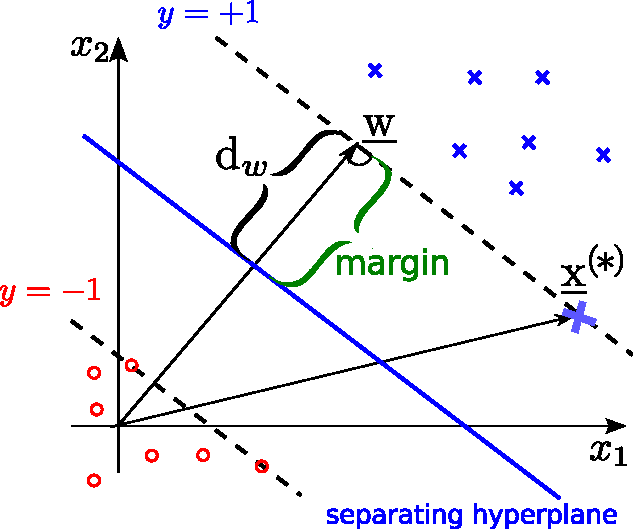
\includegraphics[height=4cm]{img/section2_fig13_v2_space} 
    \mode<article>{
    \caption{
    Binary classification setting.
    }
    \label{fig:setting}
    } 
\end{figure}
}
\mode<presentation>{
\placeimage{8.7}{2.5}{img/section2_fig13_v2_space}{width=5.2cm}
}


\begin{itemize}
	\item \underline{Data}:\\[2mm]
	$
	\Big\{ \left(\vec x^{(\alpha)}, y^{(\alpha)}_{T} \right) \Big\}_{\alpha=1}^{p}\,
	$\\[2mm]
	where $\vec x \in \R^{N}$, $y_T^{(\alpha)} \in \{-1, 1\}$\\

	\item \underline{Model}:\\[2mm]
	$
	y(\vec x; \vec w) = \sign \big( \vec w^{\top} \vec x + b \big)
	$
    
    \item \underline{Objective}:
    
    Choose the decision boundary s.t. the margin is \emph{maximal}.
    
    \item \underline{Assumption}:
    
    Perfect linear separation of both classes:
    
    In the case of a simple connectionist neuron:
    \begin{equation}
    \vec w^{\top} \vec x + b \;\;
    \left \{ \begin{array}{ll}
					\ge& 0 \;\;\text{for } {\color{blue}y_{T} = +1}\\
					<& 0 \;\;\text{for } {\color{red}y_{T} = -1}
				\end{array} \right.  
    \end{equation}
    The solution is not unique.
    
\end{itemize}
    
\end{frame}

\begin{frame}\frametitle{\subsecname}
    \mode<presentation>{
\placeimage{8.7}{2.5}{img/section2_fig13_v2_space}{width=5.2cm}
}

Let $\vec w^{*}$ and $b^{*}$ describe the optimal hyperplane that maximizes margin of separation:
    \begin{equation}
    \vec w^{*\top} \vec x + b^{*} \;\;
    \left \{ \begin{array}{ll}
					\ge& 1 \;\;\text{for } {\color{blue}y_{T} = +1}\\
					\le& -1 \;\;\text{for } {\color{red}y_{T} = -1}
				\end{array} \right.  
    \end{equation}
    
    For points that lie on the margin are characterized by:
    
    \begin{equation}
    \vec w^{*\top} \vec x + b^{*} \;\;
    \left \{ \begin{array}{ll}
					=& 1 \;\;\text{for } {\color{blue}y_{T} = +1}\\
					=& -1 \;\;\text{for } {\color{red}y_{T} = -1}
				\end{array} \right.  
    \end{equation}
    
    These points will be referred to as the \emph{support vectors}.
    
    The margin of separation between the two classes $= 2 \mathrm{d_{w}} = \frac{2}{\lVert \vec w^{*}\rVert}_{2}$
    
    Maximizing the margin $\corresponds$ minimzing the Euclidean norm of $\vec w$ (the solution to this is unique).

\end{frame}

\begin{frame}\frametitle{The primal problem}


The cost function to minimize:
    
\begin{equation}
\frac{1}{2} \vec w^{\top} \vec w = \frac{1}{2} \lVert \rVert_{2}^{2} \eqexcl \min    
\end{equation}

Minimizing the square of the norm turns it into a \emph{convex} minimization problem, which simplifies the optimization procedure.
Dividing by 2 is simply for convinience.

We want to restrict the space of solutions to that which leads to correct classification of the training points:

We therefore constrain solutions such that:

\begin{equation}
 y_{T}^{(\alpha)} \cdot \big( \vec w^{\top} \vec x^{(\alpha)} + b \big) \ge 1 \;\;\forall \alpha{}
 \label{eq:constraint}  
\end{equation}

\eqref{eq:constraint} provides a linear constraint to our optimization problem.

This gives us the \emph{primal} problem for strucuted risk minimization (SRM) prooblem.
    
\end{frame}

\begin{frame}
Applying the Lagrange method to the primal problem of SRM:

\begin{equation}
f_{0}(\vec w,b) = \frac{1}{2} \lVert \vec w \rVert_{2}^{2} = \frac{1}{2} \vec w^{\top} \vec w
\end{equation}

\begin{equation}
f_{\alpha} (\vec w,b) = -\big\{ y_{T}^{(\alpha)} \cdot \big( \vec w^{\top} \vec x^{(\alpha)} + b \big) -1 \big\} \le 1\;,\quad \alpha = 1,\ldots,p    
\end{equation}

A constraint for each data point in the training set.

The Lagrangian becomes:

\begin{equation}
L(\vec w, b, \{\lambda_{\alpha}\}) = \frac{1}{2} \lVert \vec w \rVert_{2}^{2}
- \sum_{\alpha=1}^{p} \lambda_{\alpha} \big\{ y_{T}^{(\alpha)} \cdot \big( \vec w^{\top} \vec x^{(\alpha)} + b \big) -1 \big\}
\label{ea:lagrangianprimal}
\end{equation}

Where $\{\lambda_{a}\}_{\alpha=1}^{p}$ is the set of Lagrange multipliers.

Solving the primal problem by optimizing the Lagrangian in \eqref{eq:lagrangianprimal} yields a unique solution for $\vec w$ but not for $\{\lambda_{a}\}_{\alpha=1}^{p}$ (we haven't forgotton about $b^{*}$, we will get to $b^{*}$ shortly).

\end{frame}

\begin{frame}\frametitle{From the \emph{primal} problem to the \emph{dual} problem}
    
The \emph{dual} problem: Solve the primal problem in addition to find a unique solution for the optimal multipliers.

Solution of the \emph{primal} problem:
\begin{equation}
 \vec w^{*} = \sum_{\alpha=1}^{p} \lambda_{\alpha} y_{T}^{(\alpha)} \vec x^{(\alpha)}
 \label{eq:primalsolution1}
 \end{equation}

and

\begin{equation}
 \sum_{\alpha=1}^{p} \lambda_{\alpha} y_{T}^{(\alpha)} = 0  
 \label{eq:primalsolution2}
\end{equation}

Plugging the solutions \eqref{eq:primalsolution1} and \eqref{eq:primalsolution2} back into the Lagrangian of the primal problem \eqref{eq:lagrangianprimal} yields:

\begin{align}
L(\vec w^{*}, b, \{\lambda_{\alpha}\}) &= 
\frac{1}{2} \vec w^{*\top} \vec w^{*}
- \sum_{\alpha=1}^{p} \lambda_{\alpha}  y_{T}^{(\alpha)} \vec w^{*\top} \vec x^{(\alpha)}
- \sum_{\alpha=1}^{p} \lambda_{\alpha}  y_{T}^{(\alpha)} b
+ \sum_{\alpha=1}^{p} \lambda_{\alpha}\\
&= -\frac{1}{2} \sum_{\alpha=1}^{p} \sum_{\beta=1}^{p}
\lambda_{\alpha} \lambda_{\beta} y_{T}^{(\alpha)} y_{T}^{(\beta)} {\vec x^{(\alpha)}}^{\top} \vec x^{(\beta)}
+ \sum_{\alpha=1} \lambda_{\alpha} \eqexcl \max
\end{align}

\end{frame}

\begin{frame}
Finding $b^{*}$    
\end{frame}

\begin{frame}

\question{What about non-linearly separable classes?}

kernel trick
    
\end{frame}

\subsection{C-SVM}

\begin{frame}

\question{What if the two classes are still not perfectly separable?}

- C-SVMs

No longer assume a perfect separation between the classes:

    
\end{frame}
